\documentclass[tikz,border=10pt]{standalone}
\usepackage{tikz}
\usepackage{verbatim}
\begin{document}
	\usetikzlibrary{arrows,positioning} 
	\tikzset{
		%Define standard arrow tip
		>=stealth',
		% Define arrow style
		pil/.style={
			->,
			thick,
			shorten <=2pt,
			shorten >=2pt,}
	}
	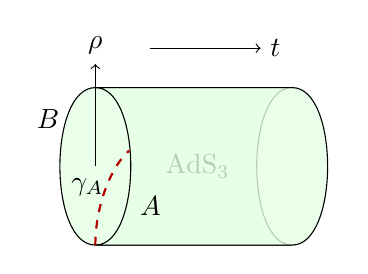
\begin{tikzpicture}
	\tikzstyle{Filling} = [fill=green!10,fill opacity=0.8]
	\filldraw[Filling] (0,0)..controls(-0.6,0)
	and(-0.6,2)..(0,2)--(2.5,2)..controls(1.9,2)
	and(1.9,0)..(2.5,0)--cycle;
	\draw (1.3,1) node{AdS${}_3$};
	\filldraw[Filling] (0,0)..controls(0.6,0)
	and(0.6,2)..(0,2)--(2.5,2)..controls(3.1,2)
	and(3.1,0)..(2.5,0)--cycle;
	\draw[->,thin] (0.7,2.5)--(2.1,2.5) node[anchor=west]{$t$};
	\draw[->,thin] (0,1)--(0,2.3)node[anchor=south]{$\rho$};
	\draw[dashed,red!70!black,thick]   (0,0)..controls(0,0.5)and
	(0.2,1)..(0.43,1.2);
	\draw (-0.1,0.5) node[anchor=south]{$\gamma_A$};
	\draw (0.7,0.5) node{$A$};
	\draw (-0.6,1.6) node{$B$};
	
	\end{tikzpicture}
\end{document}